% Desenvolvimento
% ---
\chapter[Desenvolvimento]{Desenvolvimento}
% ---
    \section{Considerações iniciais}
    Este capítulo descreve as etapas de desenvolvimento dos modelos de previsão de chances de indicação e premiação no Oscar, detalhando as escolhas realizadas e os procedimentos adotados no processo.

    \section{Atividades realizadas}

        \subsection{Obtenção dos dados}\par

        Foi escolhida como fonte de dados para o trabalho a database "The Movies Dataset", da plataforma Kaggle. Trata-se de um conjunto incluindo metadados para todos os 45.000 filmes listados no conjunto Full MovieLens. O conjunto de dados consiste em filmes lançados em ou antes de julho de 2017. Os dados incluem elenco, equipe, palavras-chave do enredo, orçamento, receita, pôsteres, datas de lançamento, idiomas, empresas de produção, países, contagens de votos TMDB e média de votos".\cite{kaggle2017}\par

        A base de dados 'The Oscar Award, 1927 - 2020' foi utilizada para complementar os metadados, adicionando a eles as informações de indicações na premiação.\cite{kaggle2019}

        \subsection{Limpeza e tratamento dos dados}\par
        
        \begin{figure}[htb]
        	\caption{\label{faltantes_film}Dados faltantes na coluna film}
        	\begin{center}
        		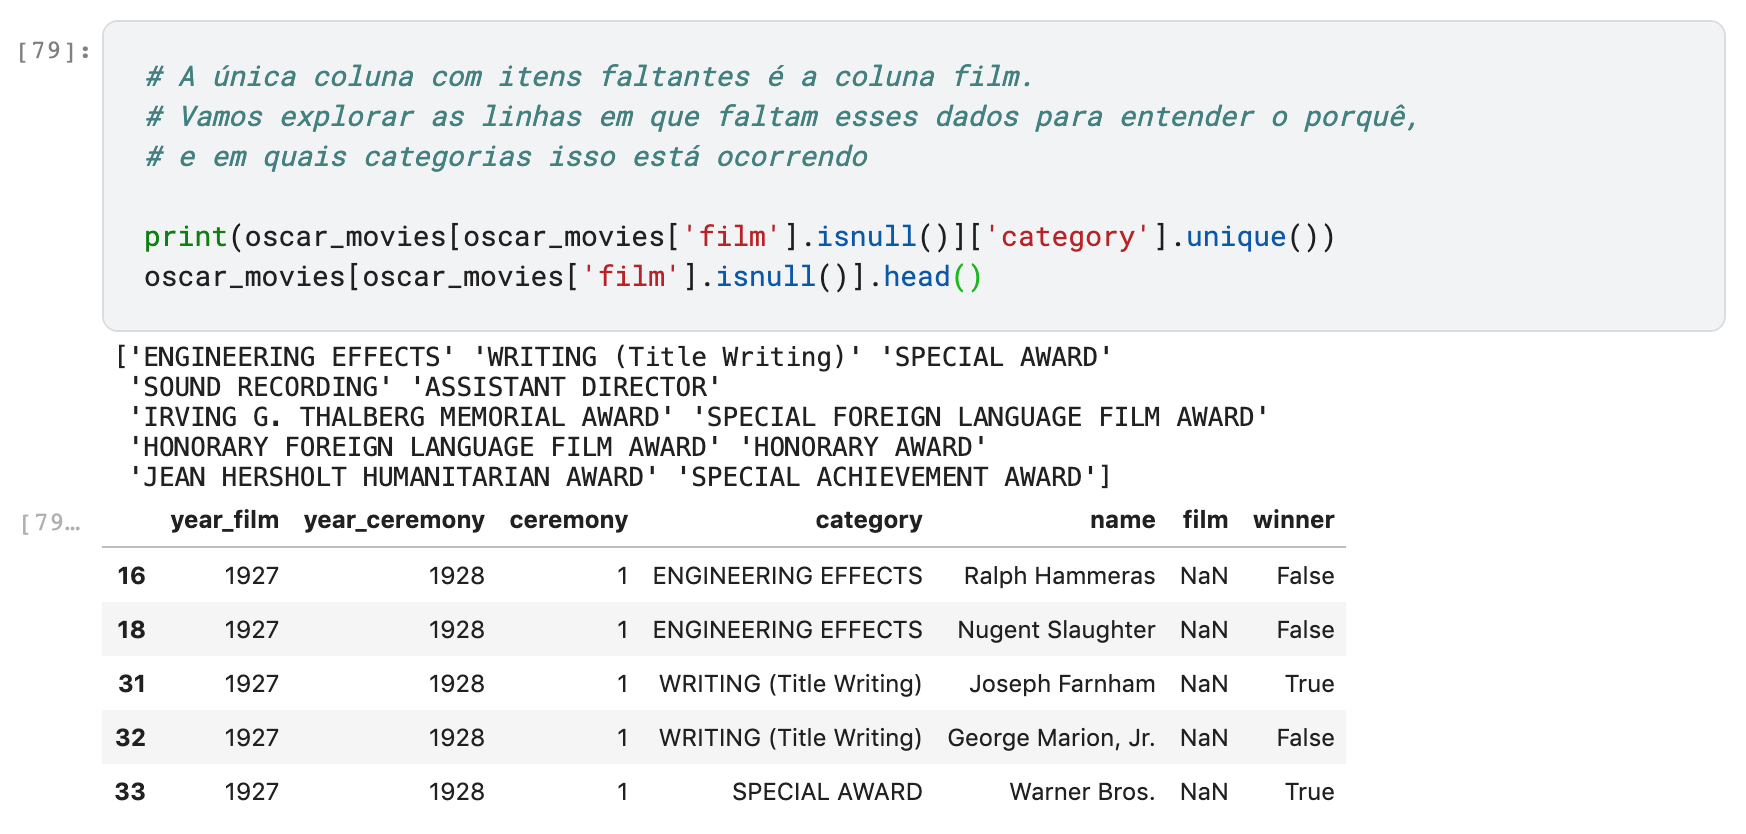
\includegraphics[scale=0.5]{faltantes_film.png}
        	\end{center}
        	\legend{Fonte: trabalho nosso}
        \end{figure}

        O primeiro desafio relacionado à limpeza e tratamento dos dados aparece na base \citeonline{kaggle2019}. Embora a base esteja bastante completa em todas os outras colunas, a coluna 'film' - justamente a que traz o nome do filme relacionado àquela premiação - está nula em 304 linhas  (figura \ref{faltantes_film}).

        Em algumas dessas categorias, nota-se que se trata de prêmios honorários, humanitários ou de conjunto da obra. Esses dados foram desconsiderados, já que não se referem a um filme específico.

        Já para duas das categorias que apresentam dados faltantes - "SPECIAL FOREIGN LANGUAGE FILM AWARD"
        e "HONORARY FOREIGN LANGUAGE FILM AWARD" -, é possível perceber que o nome se encontra na coluna 'name', precisando apenas de tratamento em alguns casos, podendo então ser transferido para a coluna "film".

        Outras linhas com dados faltantes na coluna 'film' são de obtenção difícil ou imprecisa: um assistente de direção, por exemplo, pode ter tido mais de um filme lançado num mesmo ano, o que faria a checagem dos dados restantes muito trabalhosa. Essas colunas serão ignoradas, nos deixando ao final com 10098 linhas completas no dataset.

        Um fato que pode ser observado analisando-se esses dados restantes é que algumas das categorias tiveram mudanças de nomes - como foi o caso na premiação de filme de língua estrangeira. Já outras categorias desapareceram da premiação ("melhor filme em preto e branco") ou foram incluídas. A categoria mais recente incluída na premiação é a de melhor filme de animação, criada em 2002. \cite{usatoday2002}.

        Por esse fator, iremos desconsiderar filmes anteriores a essa data. Essa abordagem tem ainda a vantade de delimitar um recorte cronológico mais coeso, permitindo a visualisação de tendências, o que seria improvável na análise total de quase 100 anos de premiação. Iremos desconsiderar ainda a premiação de edição de som (sound editing), que foi descontinuada em 2019, a única removida após o ano de 2002.\cite{deadline2020}

        Algumas dessas categorias também precisaram de consolidação, já que seus nomes apareciam de formas diferentes. Foram utilizados os nomes mais recentes.

        O passo seguinte é integrar os esquemas dos dois datasets. Para isso, vamos considerar que um filme é o mesmo nos dois datasets caso seu nome e ano apresentem correspondência. Para a análise de nome, serão observadas as colunas 'title' (em alguns casos, também a 'original\_title') do dataset de metadados, e a coluna 'film' do dataset do Oscar. 

        Para análise dos anos, foi criada no dataset de metadados uma coluna 'release\_year', extraindo o ano da coluna 'release\_date'. Esse valor será comparado com a coluna 'year\_film' do dataset do Oscar.
        
        A coluna release\_date também será eliminada em favor de uma coluna com um valor inteiro: release\_day, o número de dias desde o começo do ano até o dia em que o filme foi lançado (indo de 1 a 366). O motivo dessa transformação é a percepção comum de que filmes lançados perto do final do ano têm maiores chances de serem indicação às premiações \cite{hdsr2020}. 

        Mas para fazer essa união entre as duas tabelas, foi também necessário normalizar nomes nas duas tabelas, adicionando-se as colunas "normalized\_title" e "normalized\_original\_title". Alguns dos desafios encontrados nesse estágio foram:

        \begin{itemize}
            \item remoção de caracteres especiais e capitalização;
            \item existência, na tabela do Oscar, de filmes com título em inglês ou no original em outra língua;
            \item títulos estilizados (geralmente com pontuação no nome);
            \item filmes com anos diferentes nos dois datasets.
        \end{itemize}

        \begin{figure}[htb]
        	\caption{\label{corresp}Correspondências inexatas encontradas}
        	\begin{center}
        		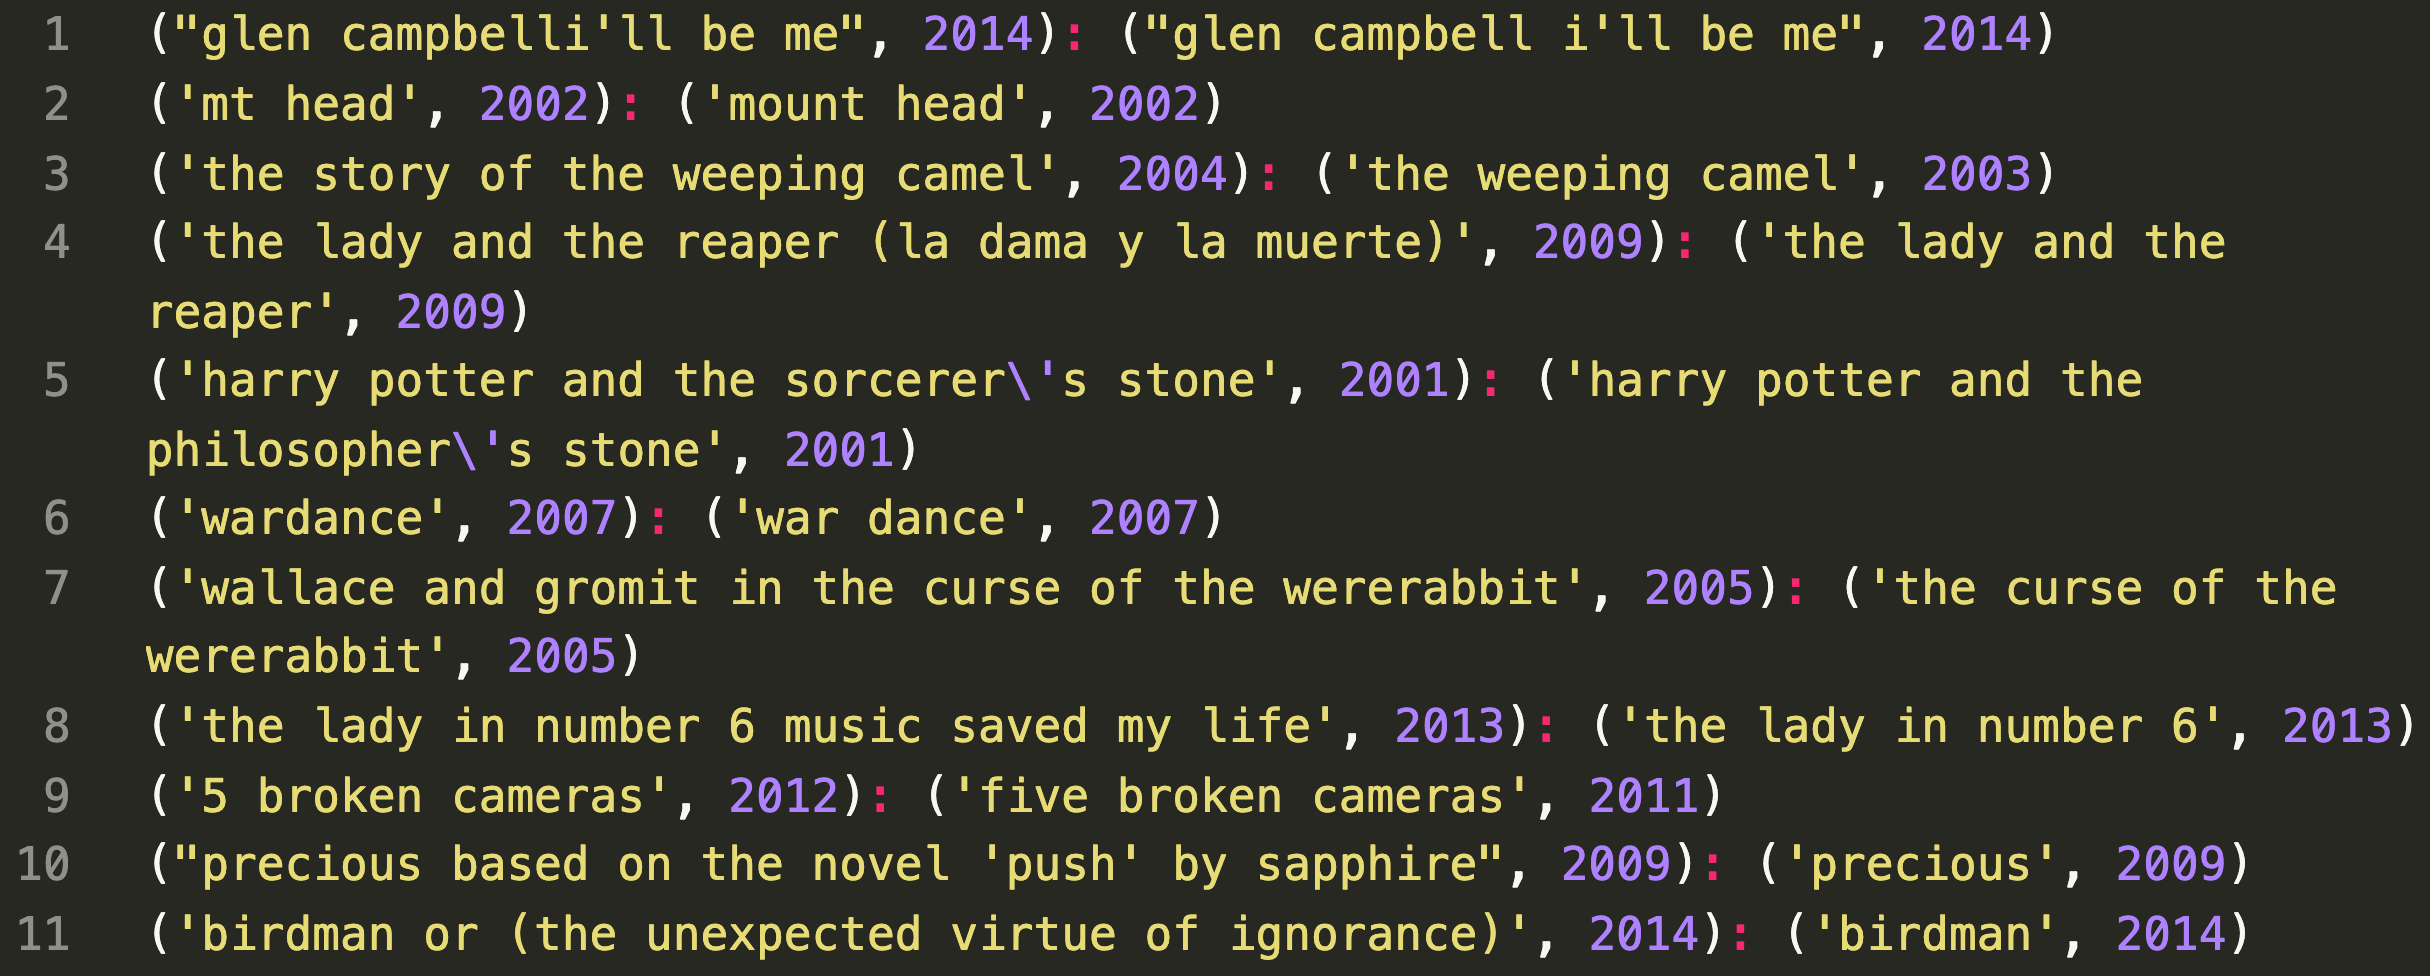
\includegraphics[scale=0.35]{corresp.png}
        	\end{center}
        	\legend{Fonte: trabalho nosso}
        \end{figure}
        
        \begin{figure}[htb]
        	\caption{\label{cat_cods}Codificação das categorias}
        	\begin{center}
        		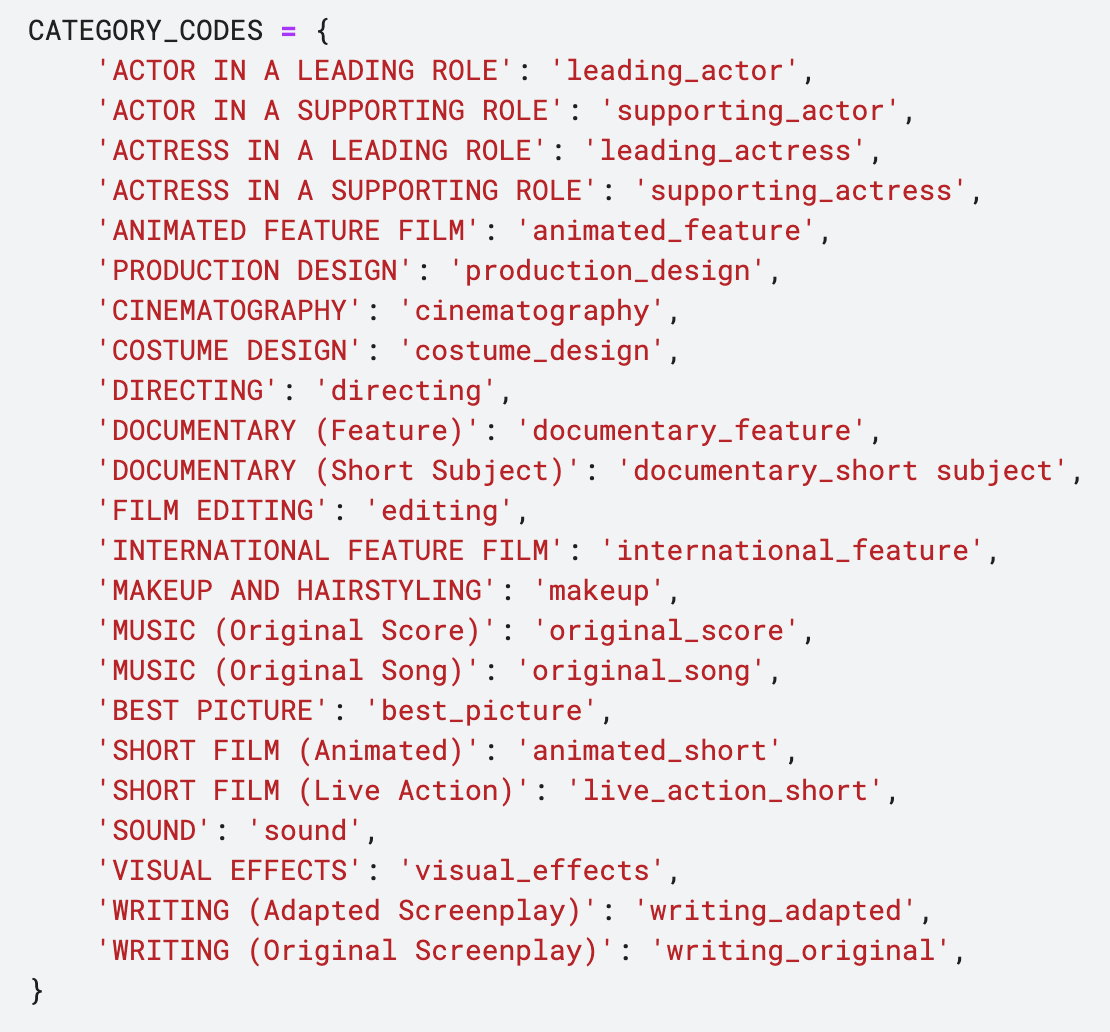
\includegraphics[scale=0.7]{categ_codes.png}
        	\end{center}
        	\legend{Fonte: trabalho nosso}
        \end{figure}

        Esse último item diz respeito à observação de filmes com ano de lançamento ('release\_year') diferentes do ano na tabela do Oscar (coluna 'year\_film'). Um exemplo é o filme 'Y tu mamá también', cuja coluna 'year\_film' tem valor 2002 no dataset do Oscar e 2001 no dataset de metadados. Foram observadas desigualdades entre os anos de até 2 anos, fato que pode estar relacionado à confusão entre as datas de produção e lançamento de um filme. Nesses casos, a coluna 'year\_film' será corrigida para o valor presente na tabela de metadados.


        Com essas informações, já é possível relacionar entre as tabelas 760 dos 942 filmes existentes no dataset do Oscar. Para os restantes 182 filmes, dois desafios especiais se deram:\par

        \begin{itemize}
            \item títulos em inglês diferentes de acordo com o país - por exemplo, o filme "Harry Potter e a Pedra Filosofal", lançado nos Estados Unidos e Índia como "Harry Potter and the Sorcerer's Stone" e nos outros países de língua inglesa "Harry Potter and the Philosopher's Stone"; \cite{yahoo2000};\par
            \item títulos divergentes entre as duas tabelas (como "Mt. Head" na tabela do Oscar, que consta como "Mount head" na tabela de metadados de filmes).\par
        \end{itemize}

        Para esses casos, foi realizada uma análise de similaridade entre os títulos não encontrados nas duas tabelas, utilizando a biblioteca nativa difflib do Python, e uma análise caso a caso.

        Nessa análise, foram encontradas outras 11 correspondências, que tiveram seus anos e nomes ajustados na tabela do Oscar (figura \ref{corresp}).

        Após essa normalização e integração de instâncias, conseguimos localizar na tabela de metadados 771 dos 942 filmes do Oscar. As informações dos demais 168 serão ignoradas.

        Podemos finalmente adicionar as informações dos Oscars ao The Movies Dataset. Para isso, vamos criar colunas no formato one-hot encoding para inserir as informações de nomeação e vitória em cada categoria para cada filme, seguindo a codificação da figura \ref{cat_cods}.

        Para cada um desses códigos, foram criadas duas colunas: '{codigo}\_nominated' e '{codigo}\_won', para designar indicação e vitória na categoria. Também foi adicionada uma coluna para indicar o ano da cerimônia em que participou o filme, com valor None como padrão.

        Após unificados os dados, pôde ser realizada análise exploratória com Pandas, Numpy, e Scikit Learn para conferir a natureza dos dados, a existência de dados faltantes ou inconsistentes e a existência de tendências que auxiliem na construção dos modelos.

        A coluna 'genres' foi convertida em one-hot encoding, resultado nas colunas: 'animation', 'comedy', 'family', 'adventure', 'fantasy', 'romance', 'drama', 'action', 'crime', 'thriller', 'horror', 'history', 'science\_fiction', 'mystery', 'war', 'foreign', 'music', 'documentary', 'western' e 'tv\_movie'.

        O mesmo processo foi aplicado nas colunas country, 'spoken\_languages' e 'original\_language', desconsiderando linguagens e países que aparecem em menos de 500 filmes.

        A coluna 'production\_companies' poderia trazer informações interessantes, já que um pequeno número de grandes produtoras detêm a maior parte das indicações e premiações \cite{argon2020}. No entanto, uma análise por one-hot encoding seria difícil nesse caso, já que mais de 15336 produtoras foram encontradas na coluna. Por conta disso, optou-se por remover também esse atributo.

        Alguns tratamentos pontuais foram realizados para modificar e padronizar os valores de algumns atributos: as colunas 'adult' (que indica se um filme é adulto), 'video' (que aponta lançamentos feitos direto para o video) e 'budget' (orçamento) foram transformadas em float.
        
        Foram localizados também 3 filmes com valores float (NaN) na coluna 'title'. Essas três instâncias parecem ter o mesmo problema: colunas desalinhadas pela falta de algum valor. Na impossibilidade de confirmar exatamente quais dados pertencem a quais colunas, vamos eliminá-las.
        
        Havia também filmes marcados no dataset como especulados, em produção, etc. Como apenas podem ser considerados ao Oscar filmes que efetivamente tenham sido lançados, checamos se algum dos filmes especulados, em produção, etc, recebeu alguma indicação ou prêmio e está com o status errado. Os outros foram descartados.
        
        Ao final do processo, algumas das colunas existentes não foram consideradas relevantes na análise e foram removidas. A saber:

        \begin{itemize}
            \item 'belongs\_to\_collection', uma representação da coleção a que supostamente pertence o filme - esse dado está representado de forma bastante subjetiva no dataset;
            \item 'homepage': link para a página oficial do filme;
            \item 'imdb\_id': identificador do filme na plataforma IMDB;
            \item 'id': identificador do filme na plataforma MovieLens;
            \item 'original\_title': título original do filme;
            \item 'overview': descrição da trama;
            \item 'poster\_path': url do poster do filme;
            \item 'tagline': frase curta utilizada na publicidade do filme;
            \item 'original\_language' (convertida em one-hot encoding)
            \item 'spoken\_languages' (convertida em one-hot encoding)
            \item 'normalized\_title' (utilizada apenas para linkar os dois datasets)
            \item 'normalized\_original\_title' (utilizada apenas para linkar os dois datasets)
            \item 'status' - diz se o filme está em pré-produção, foi finalizado, etc.
        \end{itemize}

        \subsection{Arcabouço de análise exploratória}\par

        \begin{figure}[htb]
        	\caption{\label{corrs_graph}Número de correlações maiores que cada valor de threshold}
        	\begin{center}
        		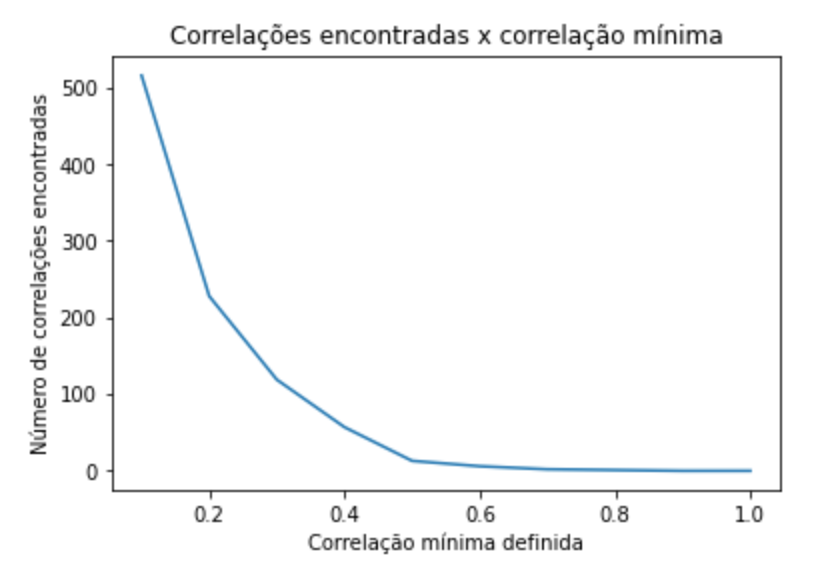
\includegraphics[scale=0.8]{corrs_graph.png}
        	\end{center}
        	\legend{Fonte: trabalho nosso}
        \end{figure}

        % \begin{figure}[htb]
        % 	\caption{\label{corrs0.4}Correlação entre colunas com valor mínimo de 0.4}
        % 	\begin{center}
        % 		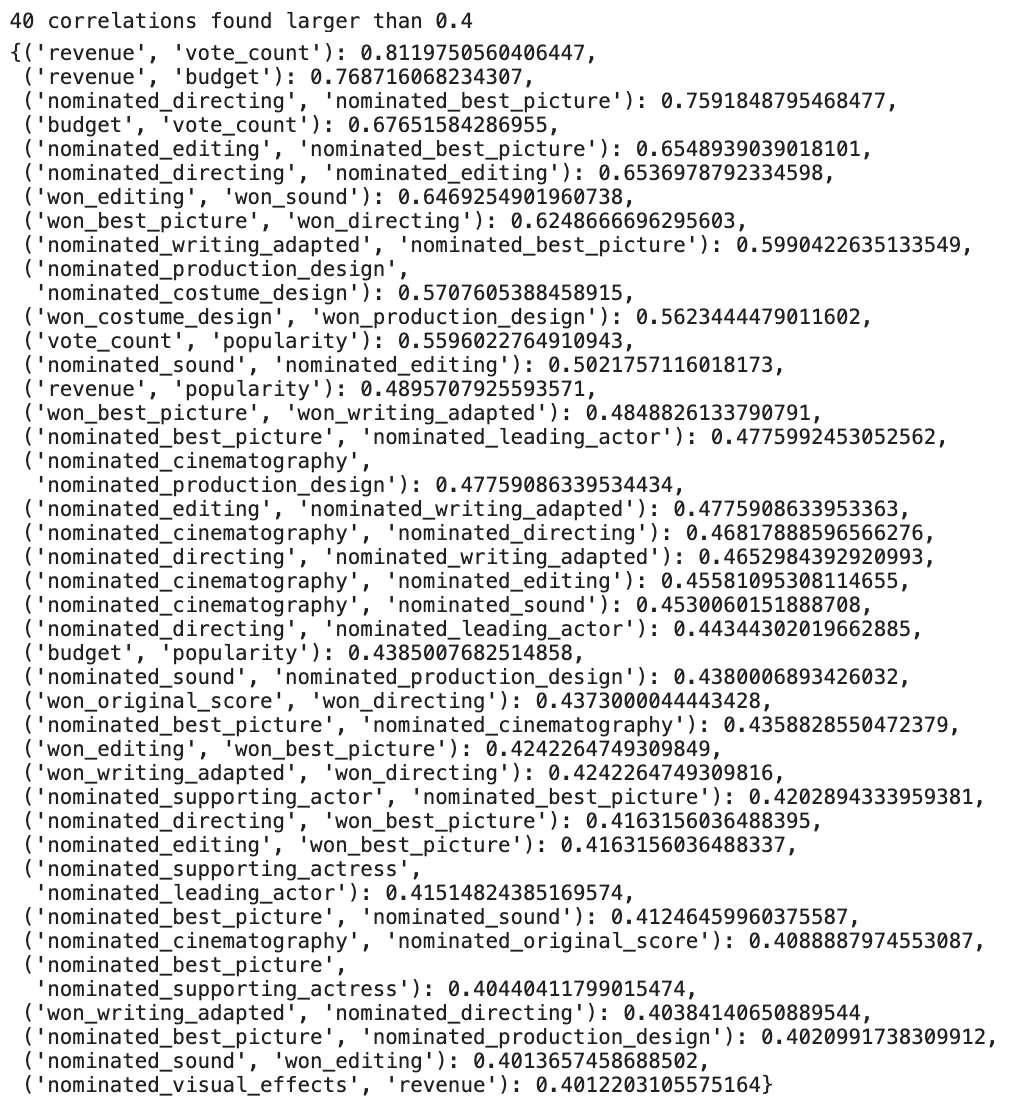
\includegraphics[scale=0.7]{corrs0.4.png}
        % 	\end{center}
        % 	\legend{Fonte: trabalho nosso}
        % \end{figure}

        % \begin{figure}[htb]
        % 	\caption{\label{vencedores_efeitos}Filmes vencedores do Oscar de Efeitos Visuais no dataset analisado}
        % 	\begin{center}
        % 		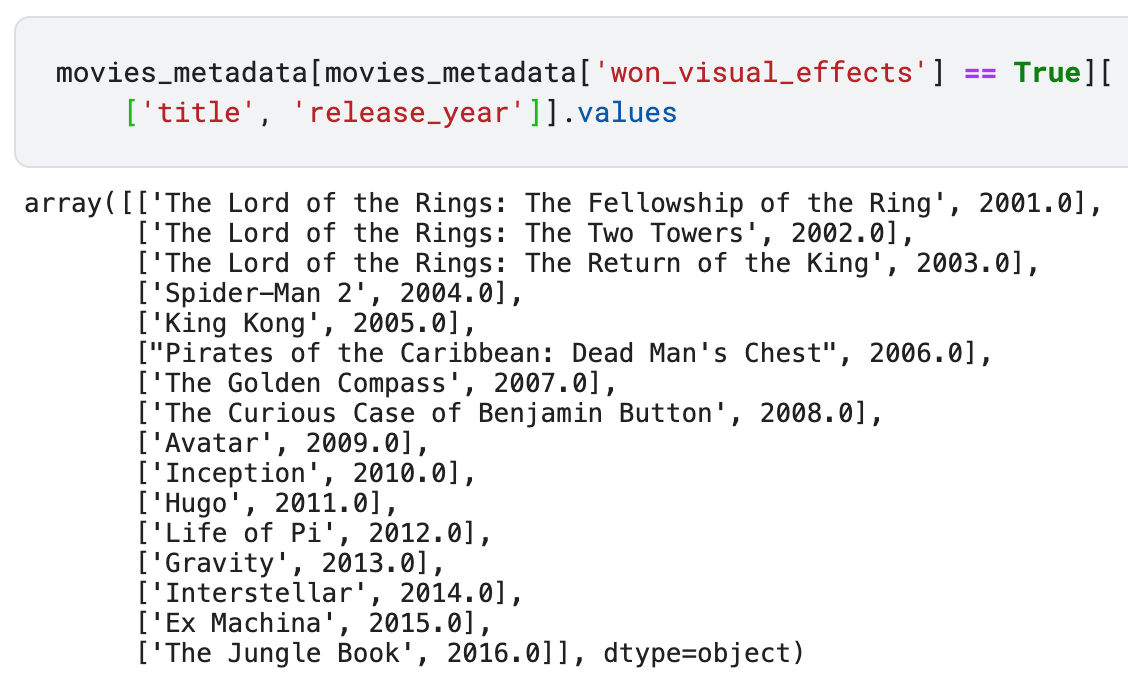
\includegraphics[scale=0.7]{vencedores_efeitos.png}
        % 	\end{center}
        % 	\legend{Fonte: trabalho nosso}
        % \end{figure}

        % \begin{figure}[htb]
        % 	\caption{\label{colunas_influentes_1}Colunas que mais aparecem nas correlações altas (inclui indicações)}
        % 	\begin{center}
        % 		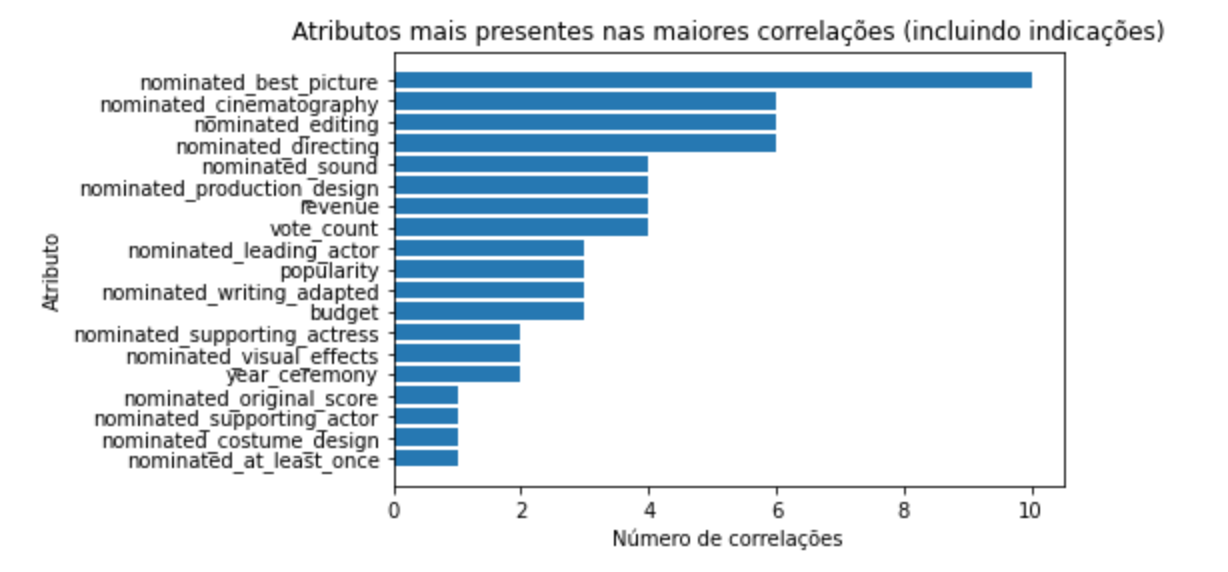
\includegraphics[scale=0.7]{colunas_influentes_1.png}
        % 	\end{center}
        % 	\legend{Fonte: trabalho nosso}
        % \end{figure}

        % \begin{figure}[htb]
        % 	\caption{\label{corrs0.4}Correlação entre colunas com valor mínimo de 0.4 - inclui indicações}
        % 	\begin{center}
        % 		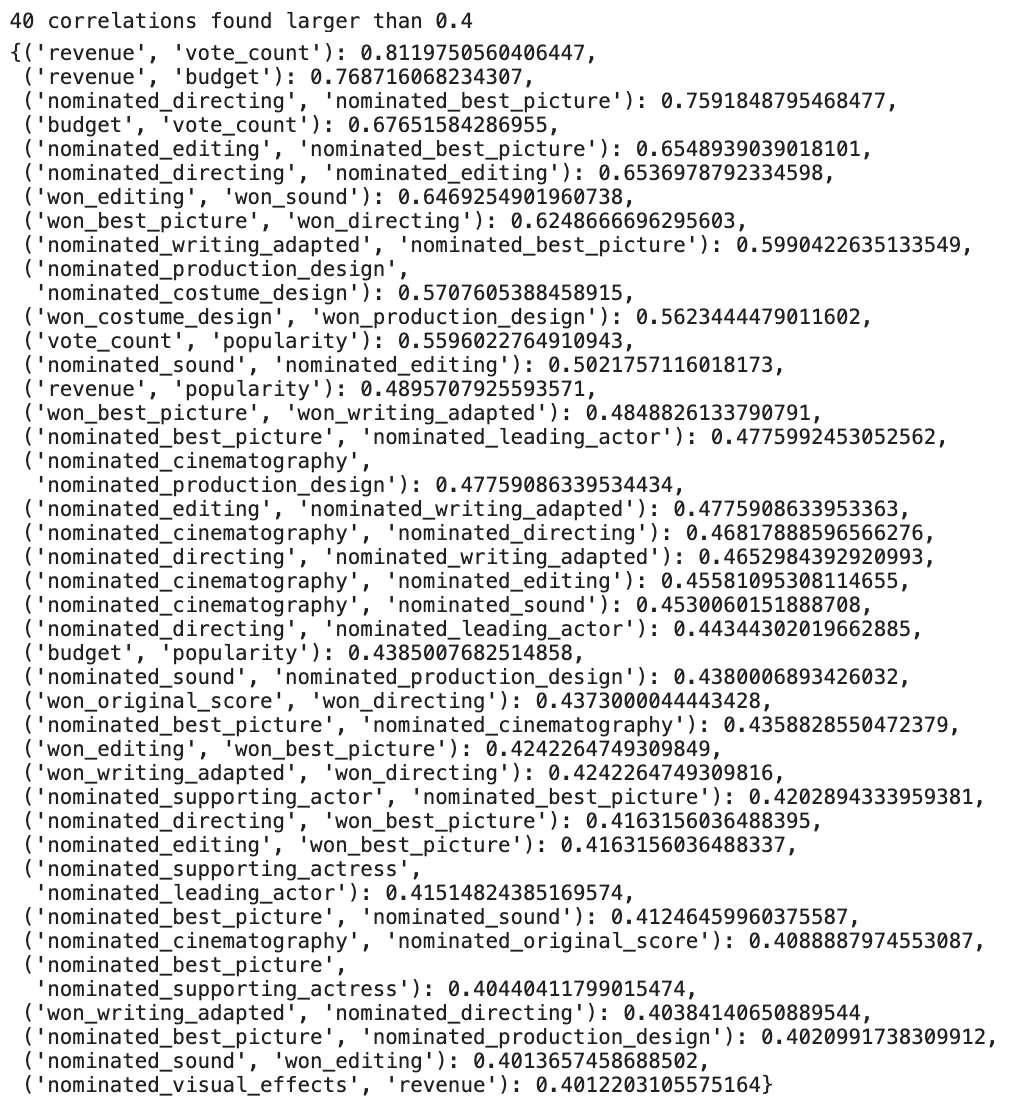
\includegraphics[scale=0.7]{corrs0.4.png}
        % 	\end{center}
        % 	\legend{Fonte: trabalho nosso}
        % \end{figure}
        
        % \begin{figure}[htb]
        % 	\caption{\label{colunas_influentes_2}Colunas que mais aparecem nas correlações altas (inclui indicações)}
        % 	\begin{center}
        % 		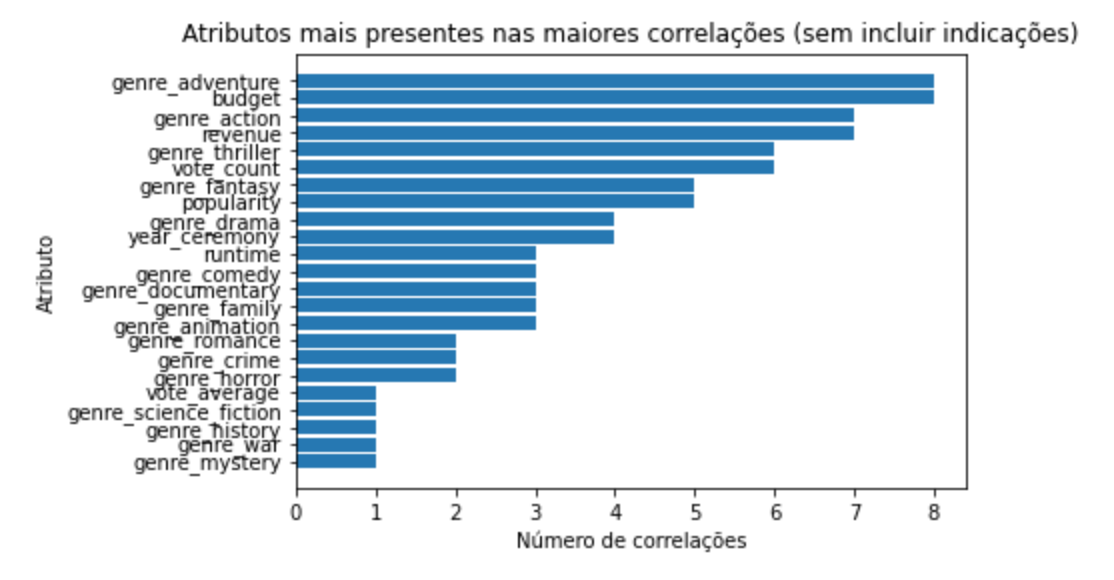
\includegraphics[scale=0.7]{colunas_influentes_2.png}
        % 	\end{center}
        % 	\legend{Fonte: trabalho nosso}
        % \end{figure}

        % \begin{figure}[htb]
        % 	\caption{\label{corrs0.15}Correlação entre colunas com valor mínimo de 0.15 - não inclui indicações}
        % 	\begin{center}
        % 		\includegraphics[scale=0.7]{corrs0.15.png}
        % 	\end{center}
        % 	\legend{Fonte: trabalho nosso}
        % \end{figure}
        
        \begin{figure}[htb]
        	\caption{\label{pca_2}Análise de componente principal em 2 dimensões - vencedores x não-vencedores}
        	\begin{center}
        		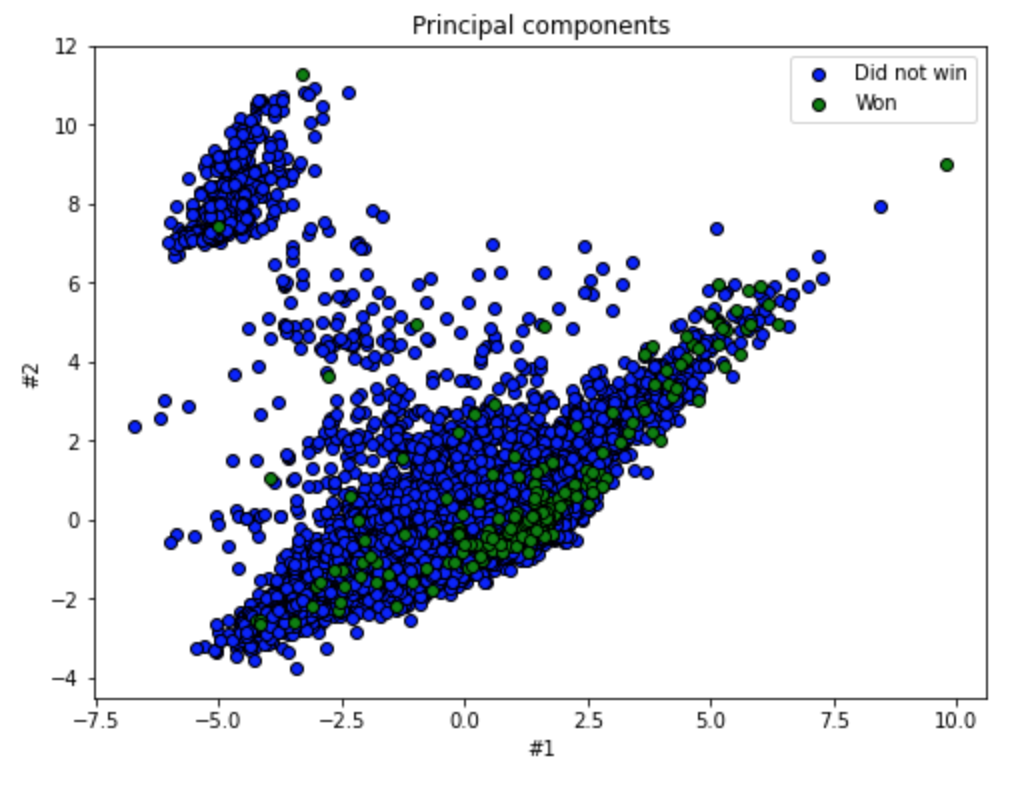
\includegraphics[scale=0.7]{pca_2.png}
        	\end{center}
        	\legend{Fonte: trabalho nosso}
        \end{figure}
        
        % \begin{figure}[htb]
        % 	\caption{\label{pca_3}Análise de componente principal em 3 dimensões - vencedores x não-vencedores}
        % 	\begin{center}
        % 		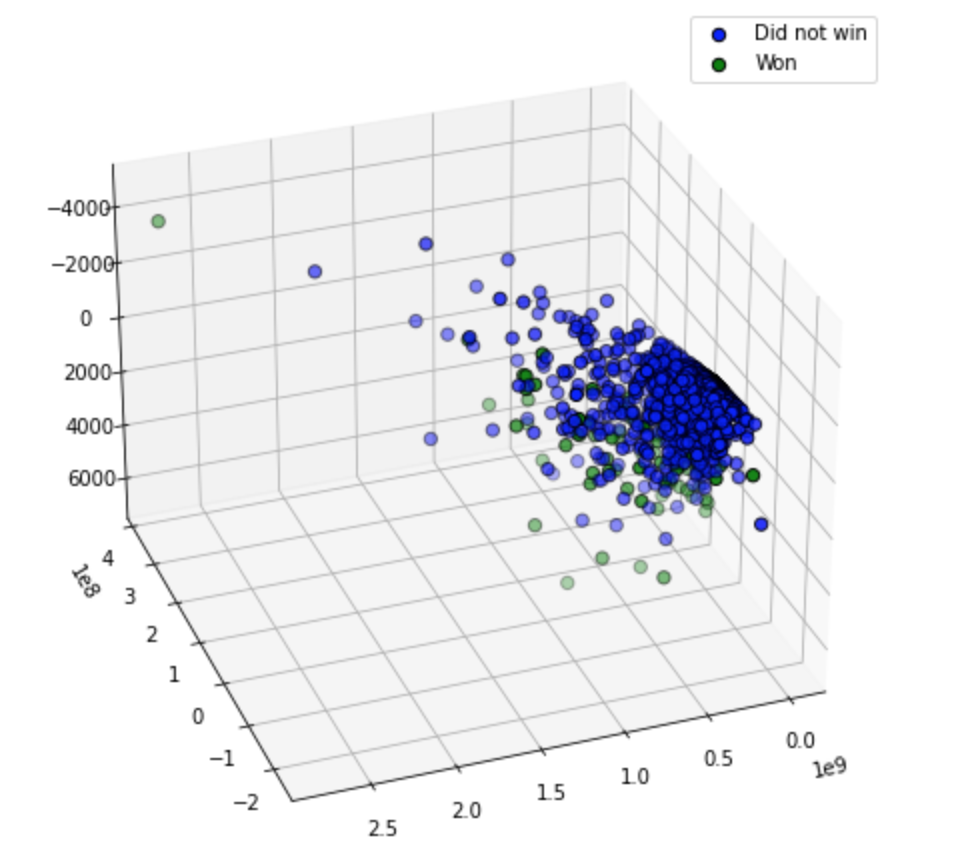
\includegraphics[scale=0.7]{pca_3.png}
        % 	\end{center}
        % 	\legend{Fonte: trabalho nosso}
        % \end{figure}
        
        % \begin{figure}[htb]
        % 	\caption{\label{outliers}Análise de outliers nos atributos numéricos}
        % 	\begin{center}
        % 		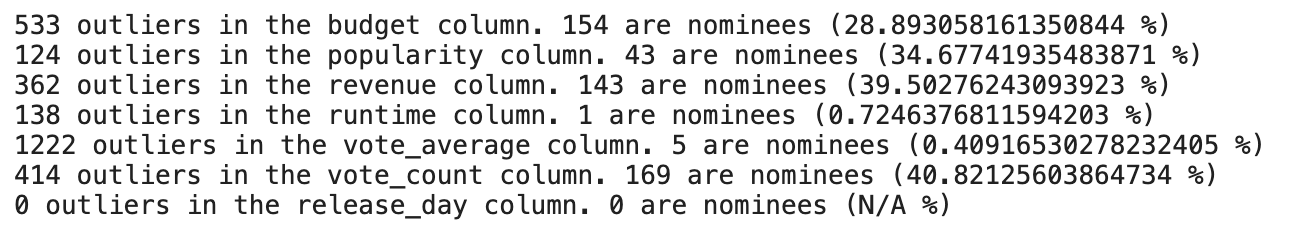
\includegraphics[scale=0.7]{outliers.png}
        % 	\end{center}
        % 	\legend{Fonte: trabalho nosso}
        % \end{figure}

        Como primeiro ponto da análise exploratória dos dados, foram analisadas as correlações entre as colunas do dataframe. Por se tratar de um grande número de atributos - aproximadamente 52, gerando um número de correlações n**2 de aproximadamente 60000 -, foi necessário experimentar valores mínimos arbitrários para as correlações.

        Também ignoramos as correlações entre países de produção. Mesmo as altas entre elas não acrescentavam dados à nossa análise. A coluna que indica filmes produzidos nas Antilhas Holandesas ('country\_AN'), por exemplo, tem correlação perfeita com a coluna que marca filmes produzidos na Polinésia Francesa ('country\_FP').\par

        Levando em conta a viabilidade da análise, decidimos nos limitar às correlações maiores do que 0.4. Correlações maiores do que 0.3 já gerariam uma lista com cerca de 100 itens (figura \ref{corrs_graph}). \par

        Algumas das correlações interessantes reveladas por essa análise, e que podem ajudar na construção dos modelos, ou indicar parâmetros importantes:

        \begin{itemize}

        \item A correlação entre orçamento de um filme e a renda gerada por ele também é muito alta.

        \item Existe grande correlação envolvendo a arrecadação de um filme é a indicação na categoria de efeitos visuais ('nominated\_visual\_effects'). Reforçamos a existência dessa relação entre arrecadação e efeitos visuais ao ver que 12 dos 16 vencedores do oscar de efeitos visuais no nosso dataset final estão na lista de 200 maiores bilheterias da história \cite{mojo2021};

        \item O atributo mais presente nas altas correlações é a coluna 'nominated\_best\_picture'. Há uma grande relação entre filmes indicados ao Oscar de melhor filme, a principal categoria da premiação, e a indicação e vitória em outras categorias.

        \item 10 correlações envolvem as colunas relacionadas ao prêmio de melhor direção ('nominated\_directing' e 'won\_directing').
        
        \end{itemize}
        
        As colunas que representam indicações ('nominated\_*') foram dominantes nessa análise. Mas é preciso levar em consideração que elas serão utilizadas como classe em uma das versões definidas do problema. Por isso, foi feita uma segunda versão da análise, desconsiderando essas colunas, para entender quais são as outras colunas que apresentam grande correlação com os outros atributos.
        
        Nessa versão, para limitar o número de correlações, foram analisadas as correlações superiores a 0.15. Dessa vez, as colunas relativas a gêneros ('genre\_*') foram predominantes.

        Realizamos também projeções, em duas e três dimensões, dos objetos do dataset, utilizando a técnica de Principal Component Analysis (PCA), utilizando cores para representar os filmes vitoriosos ou não.
        
        A representação em duas dimensões mostra um dado interessante: os filmes vitoriosos parecem se concentrar num ponto do espaço, o que pode significa uma maior chance de êxito na criação de superfícies de decisão que tragam uma resposta para o problema (figura \ref{pca_2}).
        
        \subsection{Remoção de outliers}\par
        Foi analisada a possibilidade de remoção de outliers nos atributos numéricos ('budget', 'revenue', 'runtime', e 'release\_day'), considerando-se outliers os valores a mais de 3 desvios-padrão de distância - da média dos atributos.\par
        
        A comparação da proporção de indicados ao Oscar, nossa classe de interesse, entre os outliers em cada um desses atributos mostrou que a remoção de outliers afetaria significativamente a amostragem da classe de interesse, que já é baixa. Por esse motivo, optamos por manter os outliers.

        \subsection{Seleção de atributos}\par
        
        Para permitir a obtenção de melhores resultados, além de reduzir o custo computacional do treinamento dos modelos, foi testada a redução d grande número de atributos do dataset pela regressão por stepwise. Foram utilizados thresholds de inclusão de 0.01 e de exclusão de 0.7, resultando na redução dos 97 atributos para apenas 12: 'revenue', 'release\_day', 'genre\_drama', 'country\_US', 'runtime', 'genre\_history', 'genre\_action', 'spoken\_language\_FR', 'genre\_family', 'original\_language\_EN', 'country\_FR', 'country\_IN'.
        
        Uma segunda versão do modelo foi treinada com atributos selecionados manualmente: 'revenue', 'release\_day', 'genre\_drama', 'country\_US', 'runtime'.

        \subsection{Separação em conjuntos de treinamento, validação e teste}\par
        
        Os dois modelos foram treinados e avaliados seguindo a mesma lógica de separação dos dados: 70\% são usados para treinamento dos modelos; 15\% são utilizados para validar os modelos tentar obter os melhores resultados; e os 15\% finais são guardados para sem utilizados apenas no teste final dos modelos escolhidos.
        
        Para criação desses conjuntos, foi utilizada a função "train\_test\_split" da biblioteca Scikit-learn. A função é aplicada uma vez para separação dos 70\% de treinamento, e uma segunda vez para dividir os 30 \% restantes em conjuntos em teste e validação.\newline
        
        Como os dados possuem classes desbalanceadas (uma fração muito pequena dos filmes é indicada ou vence o Oscar), todas essas operações utilizaram o parametro 'stratify'. Com esse argumento recebendo o valor True, garantimos que todos os subconjuntos criados tenham a mesma proporção de cada positivos e negativos.

        \subsection{Criação de modelos}\par
        Foram criados os seguintes modelos de regressão logística:
        
        \begin{itemize}
            \item Modelo 1: para inferir a chance de indicação na categoria Melhor Filme ("Best Picture"), treinado a partir de atributos selecionados automaticamente pelo método stepwise;
            
            \item Modelo 2: para inferir a chance de indicação na categoria Melhor Filme ("Best Picture"), treinado a partir de atributos selecionados manualmente;

        \end{itemize}
        
        \begin{figure}[htb]
        	\caption{\label{roc1}Curva ROC do modelo de predição de indicação, com seleção stepwise de atributos}
        	\begin{center}
        		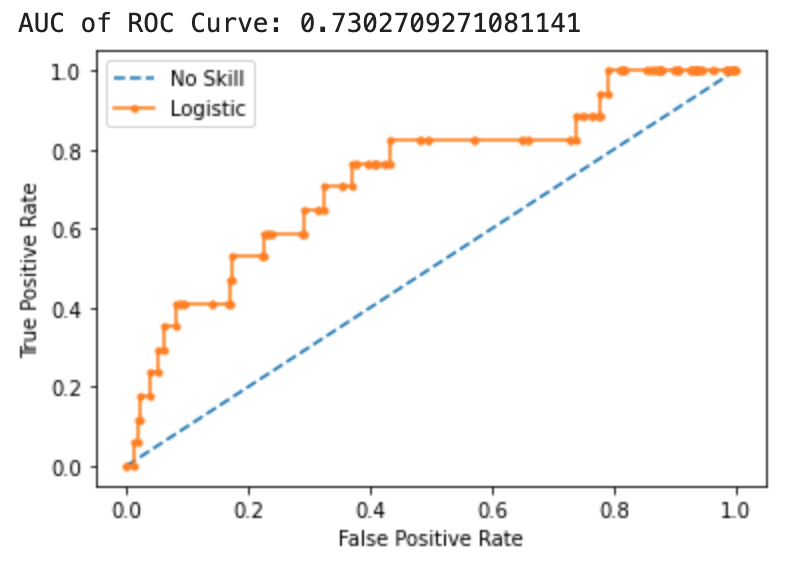
\includegraphics[scale=0.7]{roc1.png}
        	\end{center}
        	\legend{Fonte: trabalho nosso}
        \end{figure}
        
        \begin{figure}[htb]
        	\caption{\label{roc2}Curva ROC do modelo de predição de indicação, com seleção manual de atributos}
        	\begin{center}
        		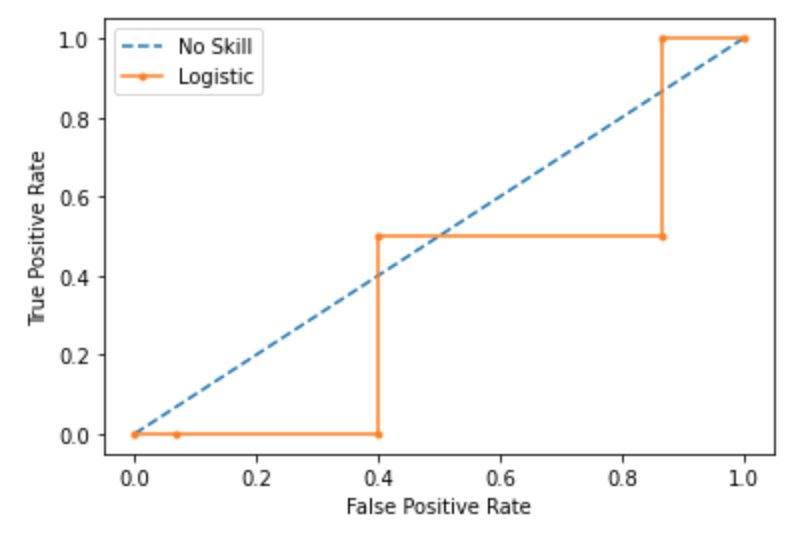
\includegraphics[scale=0.7]{roc2.png}
        	\end{center}
        	\legend{Fonte: trabalho nosso}
        \end{figure}
        
        % \begin{figure}[htb]
        % 	\caption{\label{roc3} Curva ROC do modelo de predição de vitória na categoria Best Picture, com seleção stepwise}
        % 	\begin{center}
        % 		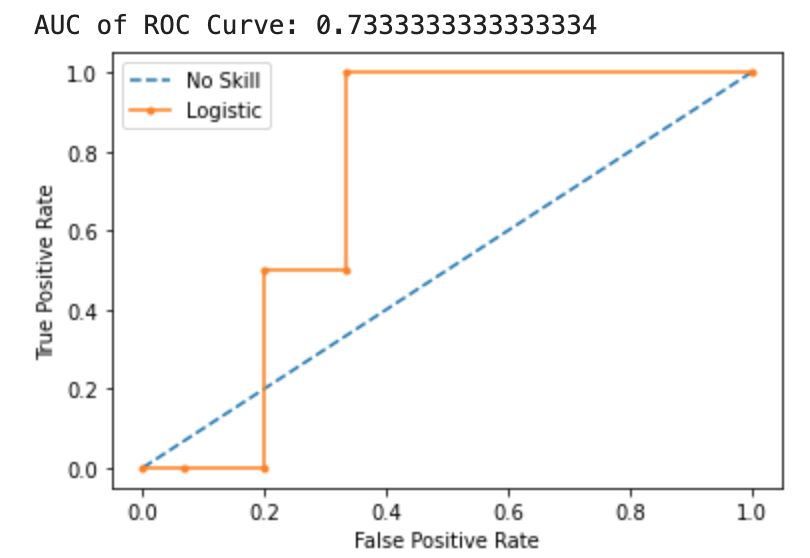
\includegraphics[scale=0.7]{roc3.png}
        % 	\end{center}
        % 	\legend{Fonte: trabalho nosso}
        % \end{figure}
        
        % \begin{figure}[htb]
        % 	\caption{\label{roc4}Curva ROC do modelo de predição de vitória na categoria Best Picture, com seleção manual de atributos}
        % 	\begin{center}
        % 		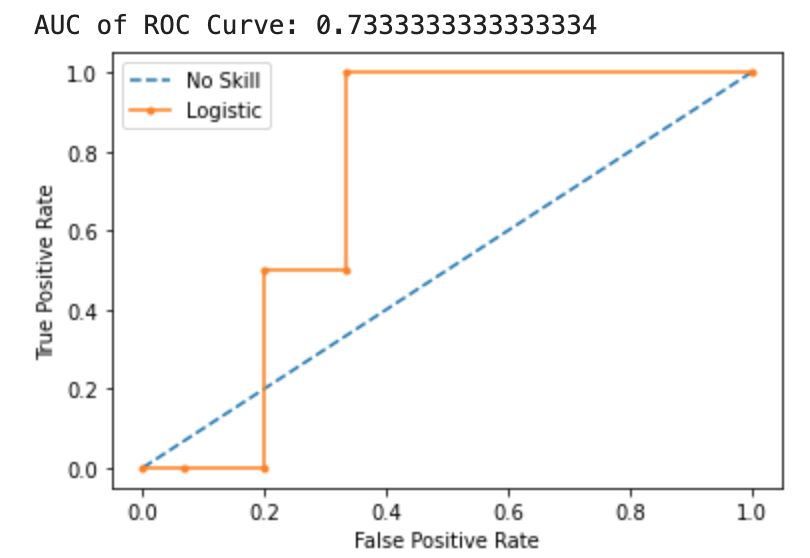
\includegraphics[scale=0.7]{roc4.png}
        % 	\end{center}
        % 	\legend{Fonte: trabalho nosso}
        % \end{figure}
        
        \begin{figure}[htb]
        	\caption{\label{confusao_1}Matriz de confusão do melhor modelo de predição de indicações}
        	\begin{center}
        		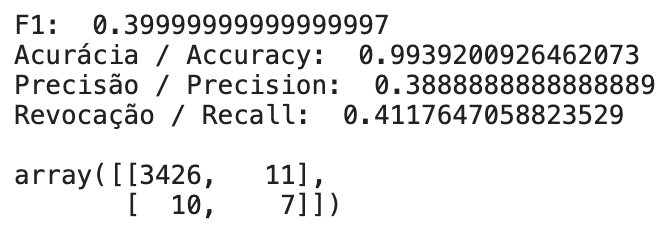
\includegraphics[scale=0.7]{confusao_1.png}
        	\end{center}
        	\legend{Fonte: trabalho nosso}
        \end{figure}
        
        \begin{figure}[htb]
        	\caption{\label{coefs_1}Coeficientes do melhor modelo de predição de indicações}
        	\begin{center}
        		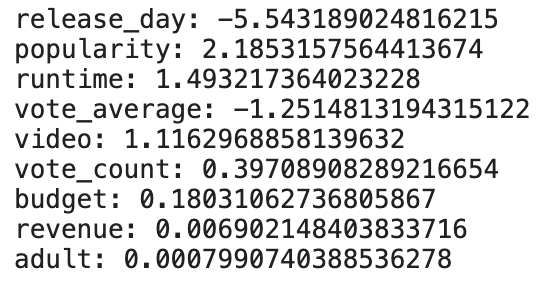
\includegraphics[scale=0.7]{coefs_1.png}
        	\end{center}
        	\legend{Fonte: trabalho nosso}
        \end{figure}
        
        Todos os modelos foram analisados por seus gráficos de curva ROC (figuras \ref{roc1} e \ref{roc2}). Como mostra a curva, o gráfico  do modelo 1 tem desempenho muito melhor que um classificador aleatório (ver \citeonline{mastery2021}). O mesmo não vale para o modelo 2, que em vários momentos tem desempenho pior que o modelo aleatório, e apenas para alguns thresholds apresenta desempenho pouquíssimo melhor.

        \subsection{Avaliação comparativa dos resultados}\par
        Para seleção do melhor threshold, foi utilizada a métrica de score f1. Incrementos de 0.01 foram feitos para thresholds entre 0 e 1, e o f1 score foi calculado para cada um dos thresholds. O threshold em que se obteve o melhor score f1 é considerado, em cada modelo, como o melhor threshold.
        
    \section{Resultados obtidos}
        
        O threshold com os melhores resultados para o modelo 1 foi de 0.15, com um f1 de 0.45. Com esse modelo, foi possível prever no conjunto de teste 7 verdadeiros positivos, com 11 falsos positivos e 9 falsos negativos, resultado bastante razoável num universo de 3454 instâncias de treinamento (figura \ref{confusao_1}).
        
        Já para o modelo 2, o melhor threshold encontrado foi de 0.33, com um f1 de 0.33. Com esse modelo, não foi possível prever no grupo de validação nenhum verdadeiro positivo, com 4 falsos positivos e 3 falsos negativos.(figura \ref{confusao_2})

        \subsection{Avaliação de importância dos metadados}\par
        A análise dos maiores coeficientes do modelo 1, em valor absoluto, revela a importância para o modelo de alguns critérios esperados, como data de lançamento, orçamento e renda. Alguns fatores menos óbvios que tiveram impacto no treinamento foram duração, se o filme foi lançado em vídeo, e se o filme é adulto ou não.(figura \ref{coefs_1})\par
        
        Para o modelo 2, em valor absoluto, os fatores que mais influenciaram o modelo foram, nessa ordem: se o filme foi lançado em vídeo, duração, média dos votos no Movie Lens, renda, popularidade no Movie Lens, adulto ou não-adulto e. orçamento.(figura \ref{coefs_2})\par